\section{Battling Track Competition Results}
\label{sec:track1-full-results}


The Battling Track competition was divided into a \textbf{Practice Stage}, \textbf{Qualifying Stage}, and \textbf{Tournament Stage}. In each phase, participating teams could compete in one or both of the Gen 1 OU and Gen 9 OU battling rulesets. The Practice and Qualifying Stages were most similar to the evaluation setup of the permanent PokéAgent Challenge leaderboard: teams connect their agents to our AI-focused Showdown server and compete in ranked battles against both their fellow participants and a large set of ``organizer baselines'' maintained by our team. Our baselines ensure accurate ratings by creating a shared set of opponents and maintaining battle activity when few participants are online. During the NeurIPS competition, organizer baselines also served as a form of held-out evaluation; some were released as part of the official starter kit, while others were kept private, so the only way to evaluate against them was to compete on the leaderboard.



\subsection{Practice Stage}
For most of the competition (July--October), participants were free to compete on the leaderboard to iterate on their solutions. Teams could create unlimited usernames to reset their ratings and evaluate new methods. A hackathon event in September reset the leaderboard and offered compute credit prizes to the top teams $36$ hours later, which were \texttt{ED-Testing} (Gen 9 OU) and \texttt{srsk-1729} (Gen 1 OU). In total, participants played about $75$k battles during the practice stage.


\subsection{Qualifying Stage}

In late October, our leaderboards were reset, and participation was restricted to one username per registered team. Teams competed to qualify for a spot in the Tournament Stage, where all teams would be guaranteed a cash prize. Qualifications were awarded to the top two teams by Elo and the next six highest by FH-BT, which is considered the more accurate metric (Appendix \ref{sec:rating-analysis}). This structure was a compromise that encouraged participation by allowing a late comeback, as Elo can be improved regardless of earlier results, and FH-BT required a minimum sample of $250$ battles, which could have been prohibitively expensive for some methods. 



The main Qualifying Stage results were presented in Figure \ref{fig:neurips_track1_main_text}. Participants played a total of 35K battles over the two-week qualifying period, and we found strong alignment across all of our skill rating metrics; Figure \ref{fig:track1_qualifying_scatter_appendix} visualizes the leaderboard across several alternatives. Figure~\ref{fig:winrates} presents head-to-head win rates among the top non-baseline participants. 

Our set of organizer baselines helps give the participant results context by grounding them against methods whose training details and performance relative to human players are known. The distinction between public and private organizer baselines created a clear separation point on both leaderboards: many participants clustered slightly above the best public baseline, whereas participants competitive with the private baselines separated from the field and qualified for the tournament. In Gen 9 OU, \texttt{FoulPlay} outperformed private baselines by all metrics, while \texttt{Q}, \texttt{PA-Agent}, and \texttt{piploop} formed a chase pack situated between the best public and private baselines. In Gen 1 OU, \texttt{4thLesson} separated from the public baselines while \texttt{PA-Agent} fell just short of the best private baselines and placed first among participants by a wide margin. 

As discussed in Section~\ref{sec:neurips}, all top-performing submissions employed RL or search-based methods rather than pure LLM approaches. Our baselines revealed systematic LLM reasoning failures---including ``panic behavior'' and other failure modes---discussed in Section~\ref{sec:neurips} and Appendix~\ref{sec:extended-discussion}. Additionally, LLM agent performance on the competition ladder was deflated by time pressure: agents frequently switched to less sophisticated fallback methods when low on time, or lost on time entirely. We have since introduced a separate long-timer leaderboard to isolate reasoning ability from inference speed (Section~\ref{sec:track1:evaluation}).



\begin{figure}[h!]
    \centering
    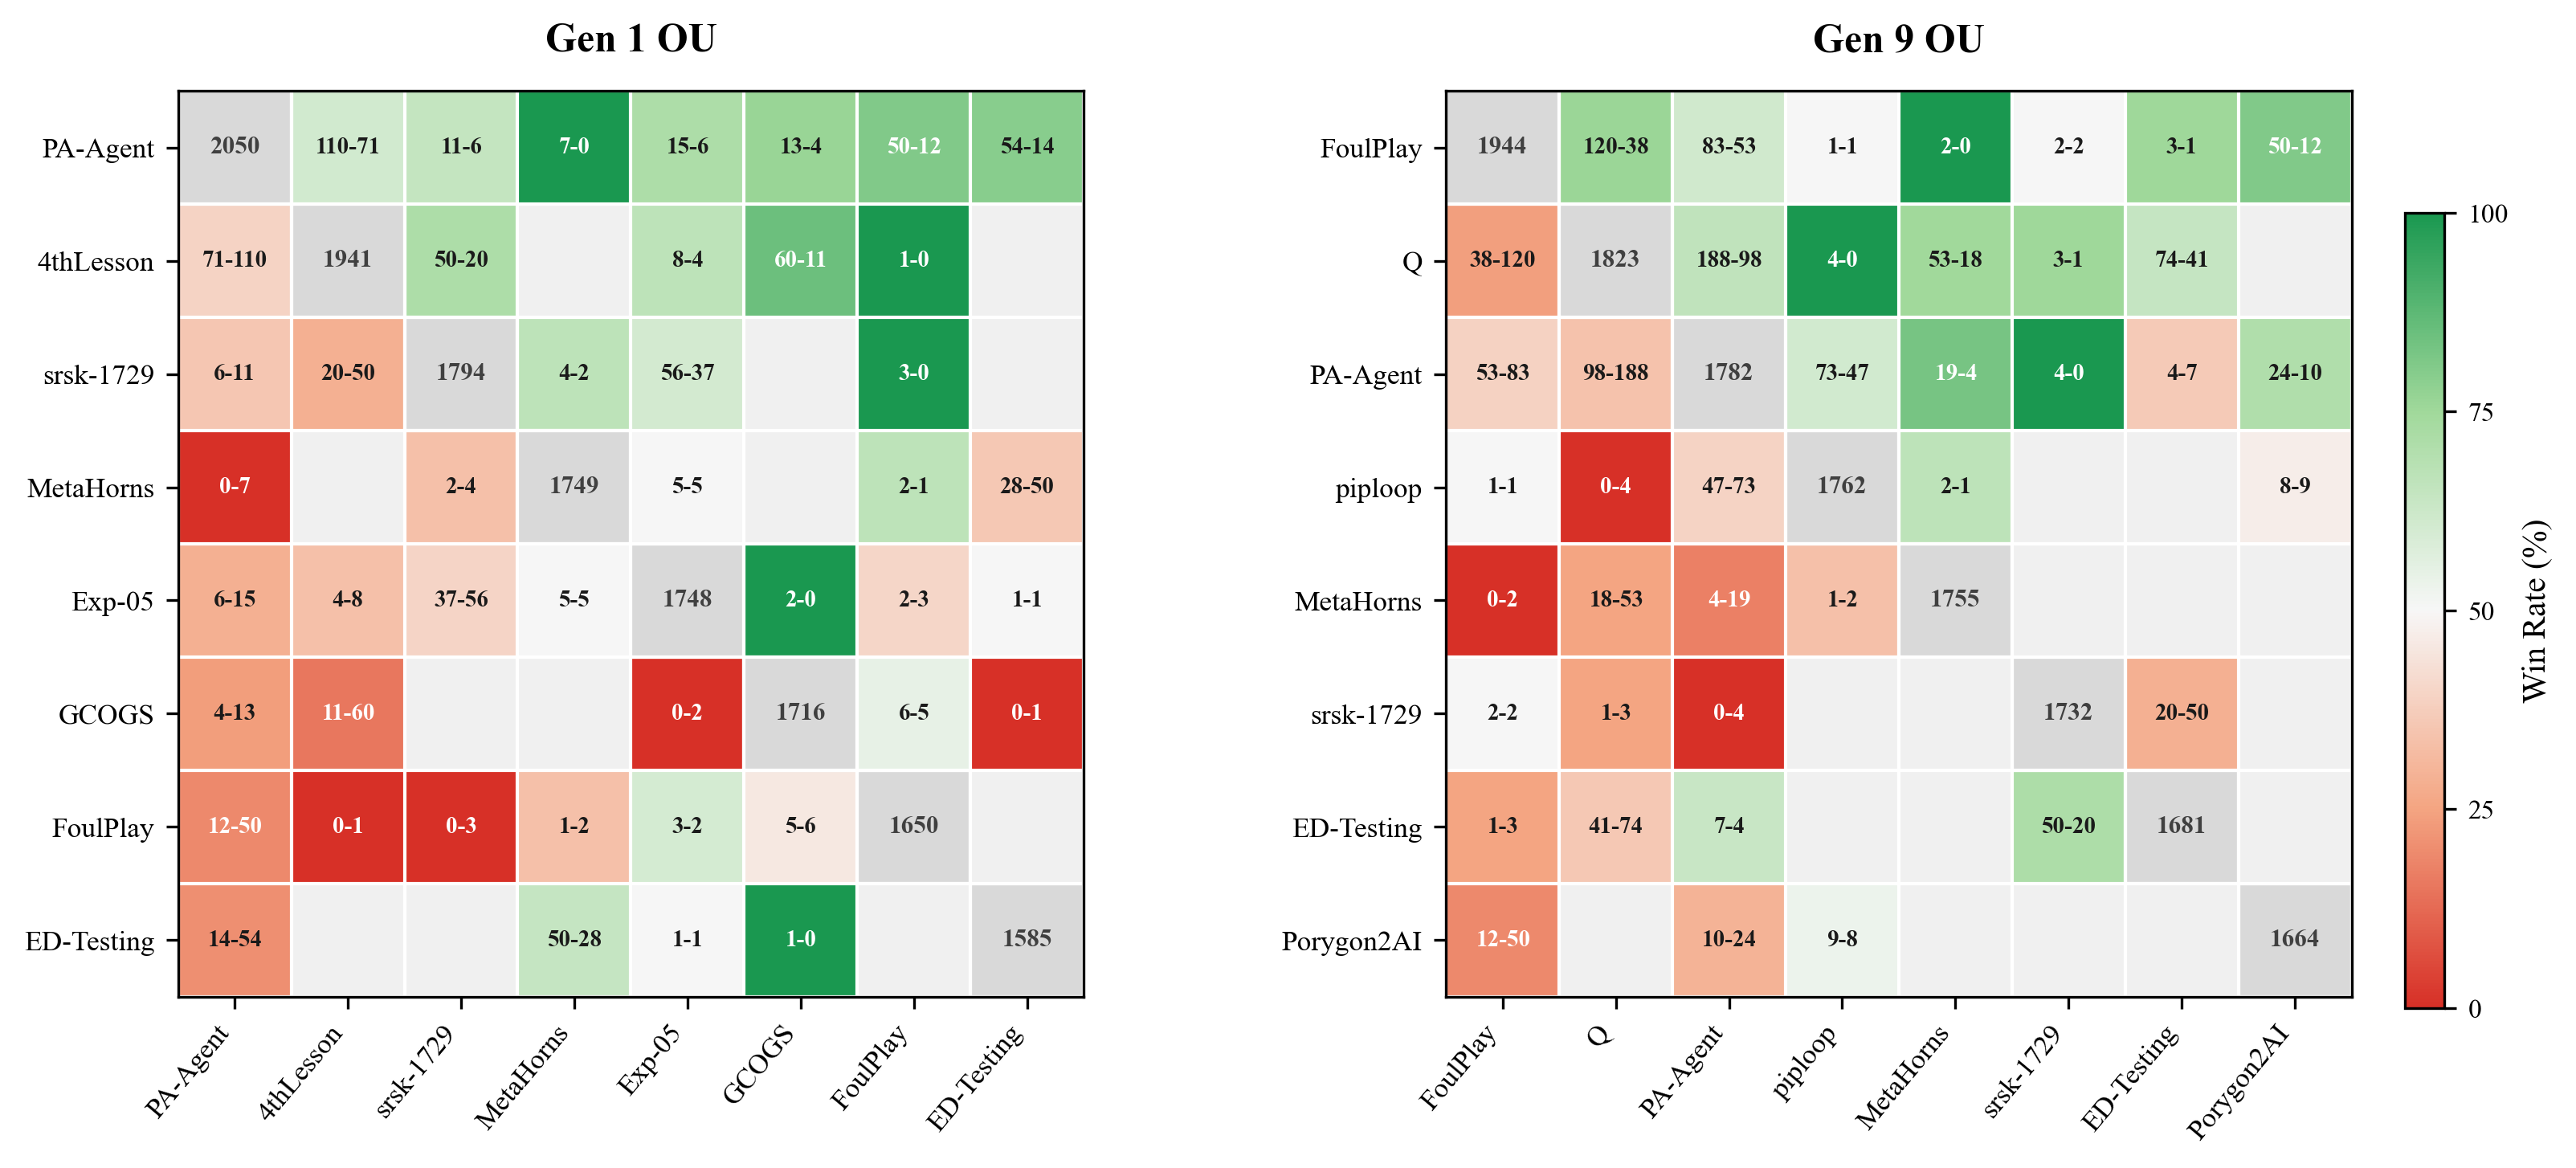
\includegraphics[width=.95\linewidth]{figures/track1_h2h.png}
    \caption{\textbf{Head-to-Head Win Rates Among Top Participants.} Heatmap matrices showing pairwise win rates for Gen 1 OU (left) and Gen 9 OU (right). Each cell shows the row player's win--loss record against the column player. Diagonal cells show each player's Elo rating. Players are ordered by Elo (highest at top). Empty cells indicate insufficient direct head-to-head matchups.}
    \label{fig:winrates}
\end{figure}


\subsection{Tournament Stage}

The competition concluded with a head-to-head single-elimination tournament among the qualifying teams, seeded by Qualifying Stage leaderboard position. Teams played their designated opponent in a best-of-99 battle match (first to 50 wins). Figure~\ref{fig:tournament} shows the tournament brackets for both formats. \texttt{PA-Agent} dominated Gen 1, defeating \texttt{4thLesson} 50--28 in the finals. In Gen 9, \texttt{FoulPlay} swept through the competition, defeating \texttt{Q} 50--14 in the finals after a close match with \texttt{PA-Agent} in the semifinals. Both tournament winners were ranked \#1 on the Qualifying Stage leaderboard and were therefore the \#1 seeds. Appendix \ref{sec:participant-methodologies} provides technical details of the first and second place methods as written by the teams themselves.

\begin{figure}[h!]
    \centering
    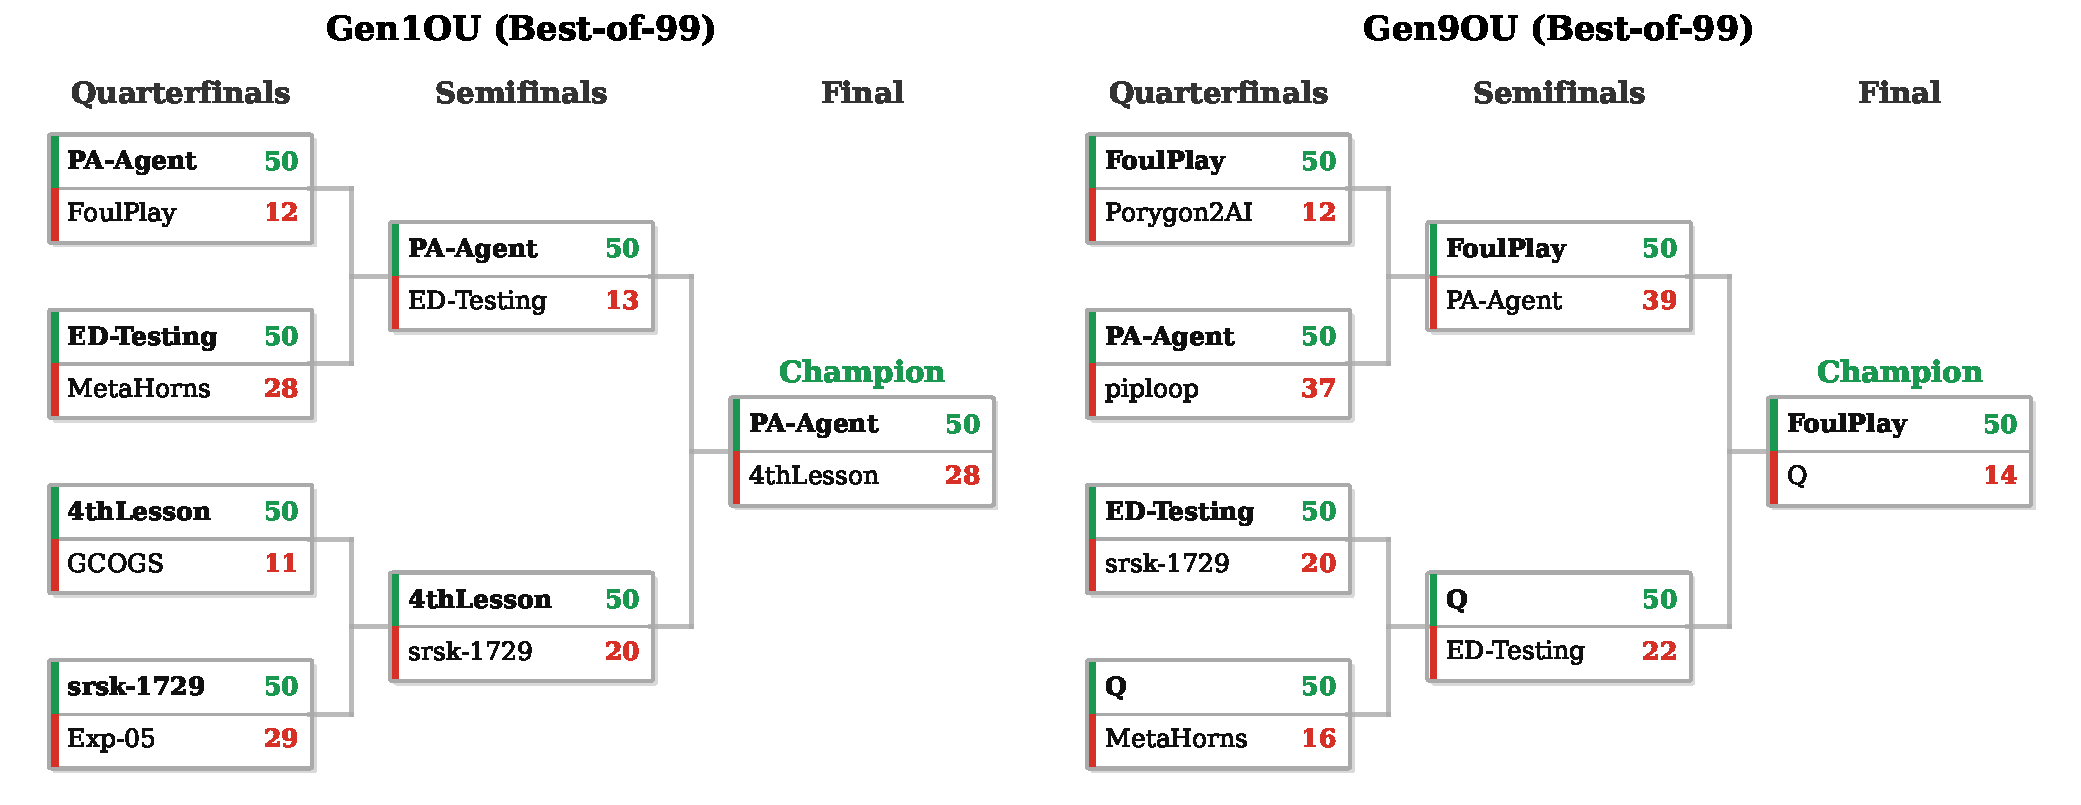
\includegraphics[width=0.98\linewidth]{figures/gen9_tournament.pdf}
    \caption{\textbf{Tournament Brackets.} Best-of-99 single-elimination brackets for Gen 1 OU (left) and Gen 9 OU (right). Numbers indicate games won by each team; green highlighting indicates winners.}
    \label{fig:tournament}
\end{figure}

\subsection{Rating System Analysis}
\label{sec:rating-analysis}

Most LLM evaluation arenas use Bradley--Terry models (batch MLE) without reporting uncertainty---a potentially misleading practice. We stress-tested four ranking systems (Bradley--Terry, Elo, Glicko-1, and GXE) across 1.6M+ agent matches (Figure~\ref{fig:rating_systems}). Top-3 agents converged across all methods (with 250+ games each), but ranks 4+ showed systematic disagreement---Elo diverged from Bradley--Terry even when error bars did not overlap. Glicko-1 offered the best tradeoff: online updates for real-time leaderboards with convergence guarantees matching batch MLE. We prefer Glicko-1 over raw Elo for agent evaluation, particularly when sample sizes vary across agents. Figure \ref{fig:track1_qualifying_scatter_appendix} compares the Battling Track competition results according to alternative skill metrics (Showdown's Elo, GXE, Win Rate) and sample size (Battles Played).

\begin{figure}[h]
    \centering
    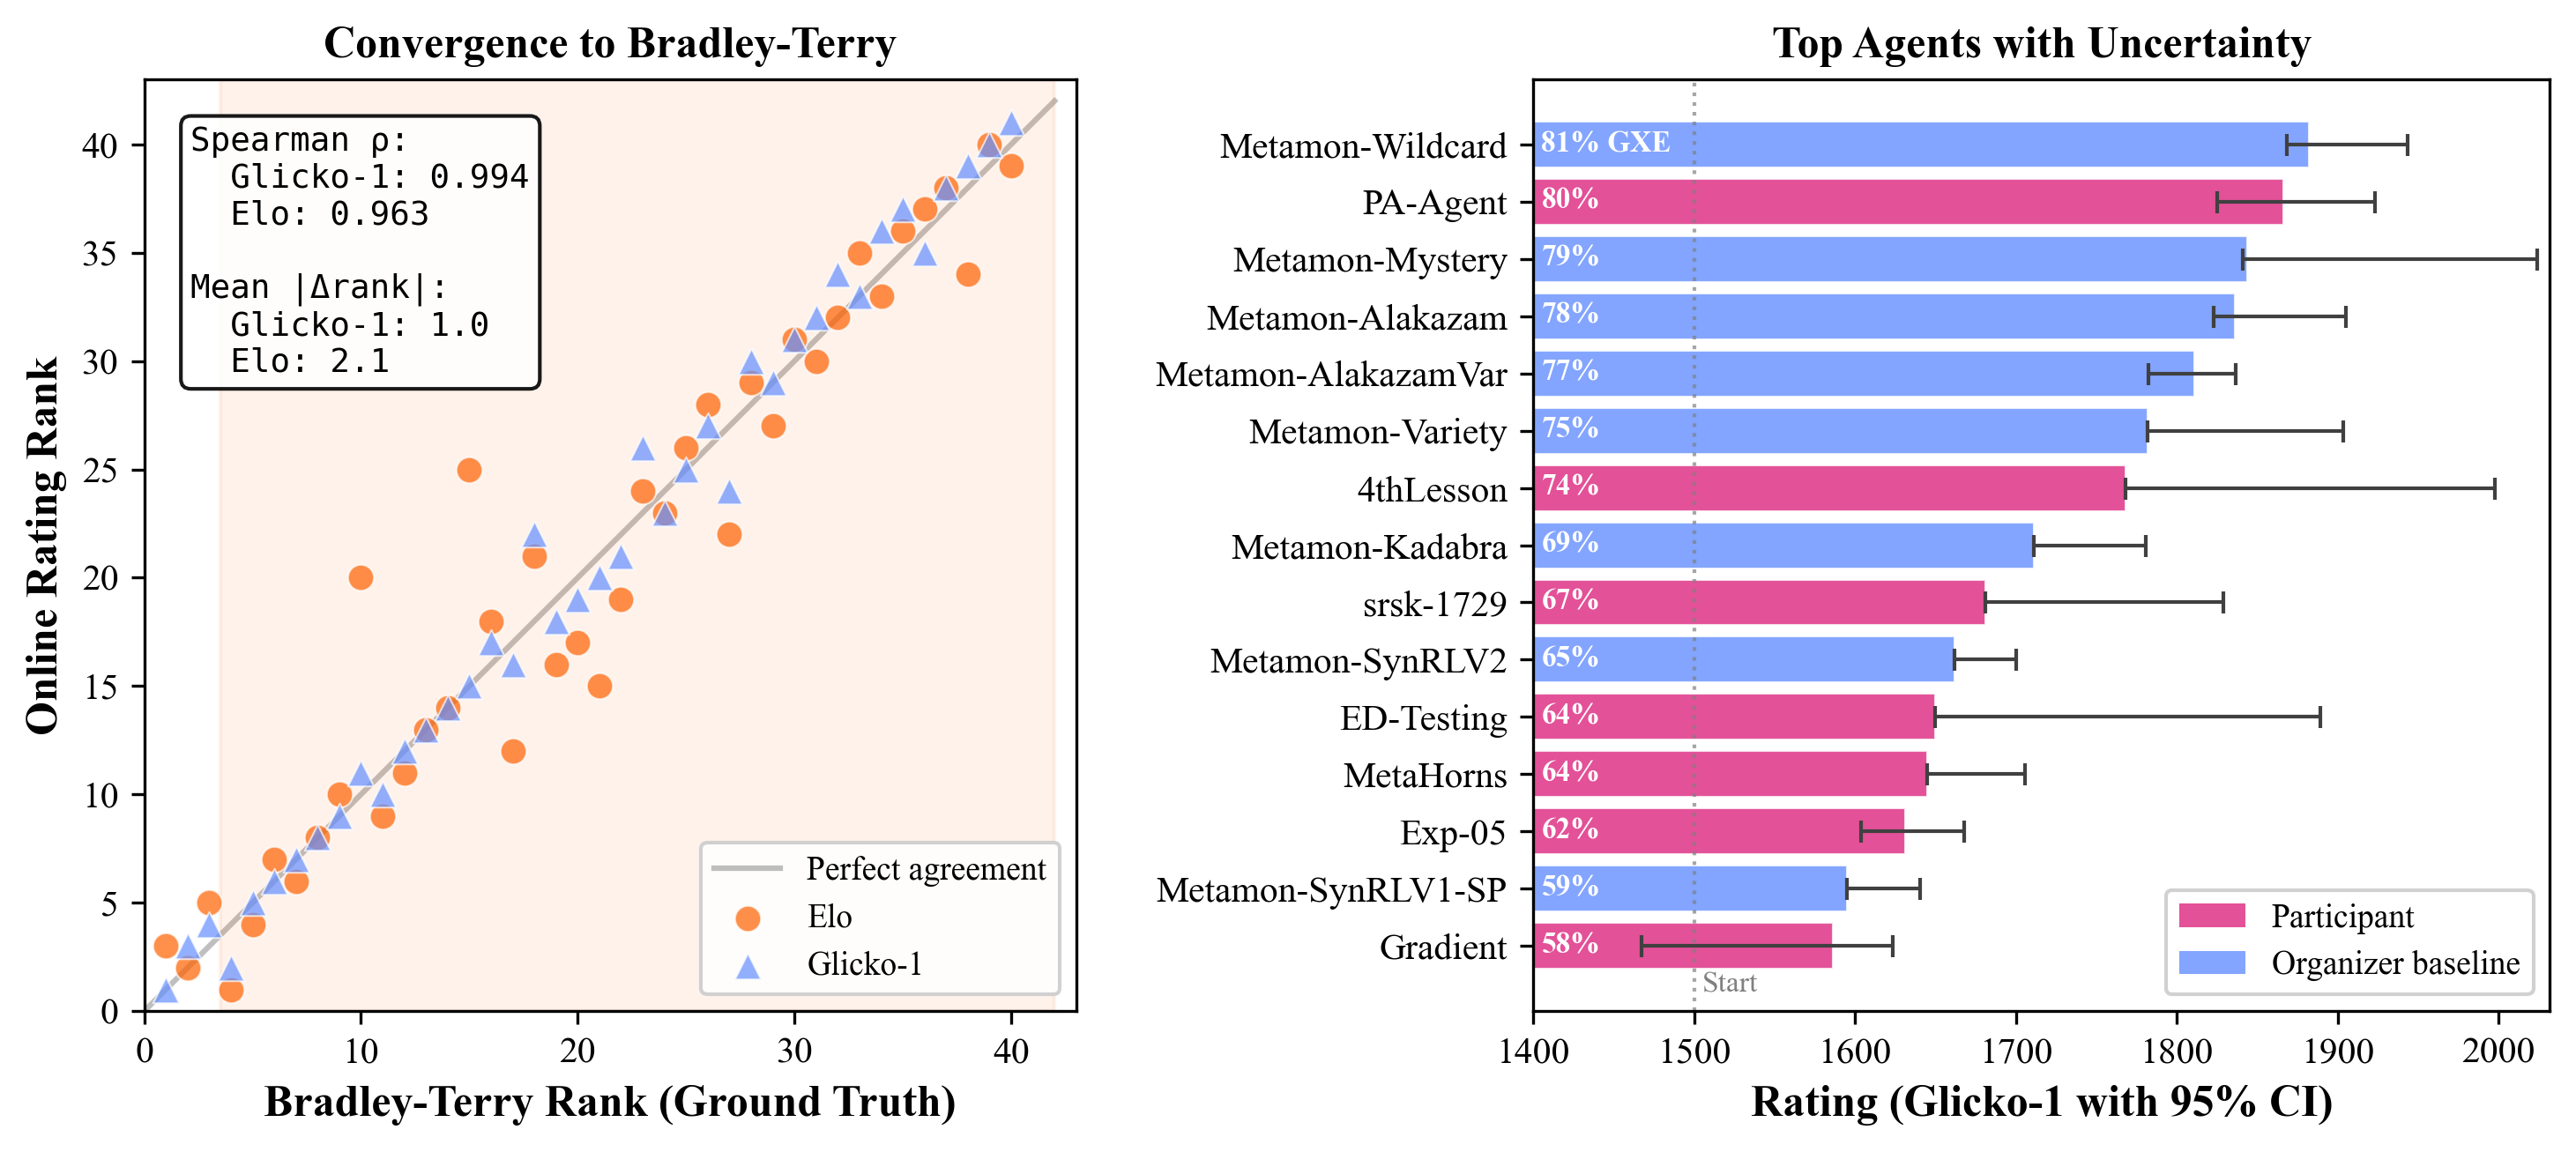
\includegraphics[width=0.95\linewidth]{figures/rating_systems.png}
    \caption{\textbf{Rating System Comparison Across 1.6M+ Matches.} Four ranking methods applied to Battling Track data. Left: Rank correlation between methods, showing Glicko-1 converges to Bradley--Terry (batch MLE) while Elo diverges for mid-ranked agents. Right: Rating trajectories with uncertainty bands for selected agents, demonstrating Glicko-1's uncertainty quantification. Top-3 agents (shaded) show consistent rankings across methods; ranks 4+ exhibit systematic disagreement, particularly between Elo and Bradley--Terry.
    }
    \label{fig:rating_systems}
\end{figure}


\begin{figure}
    \centering
    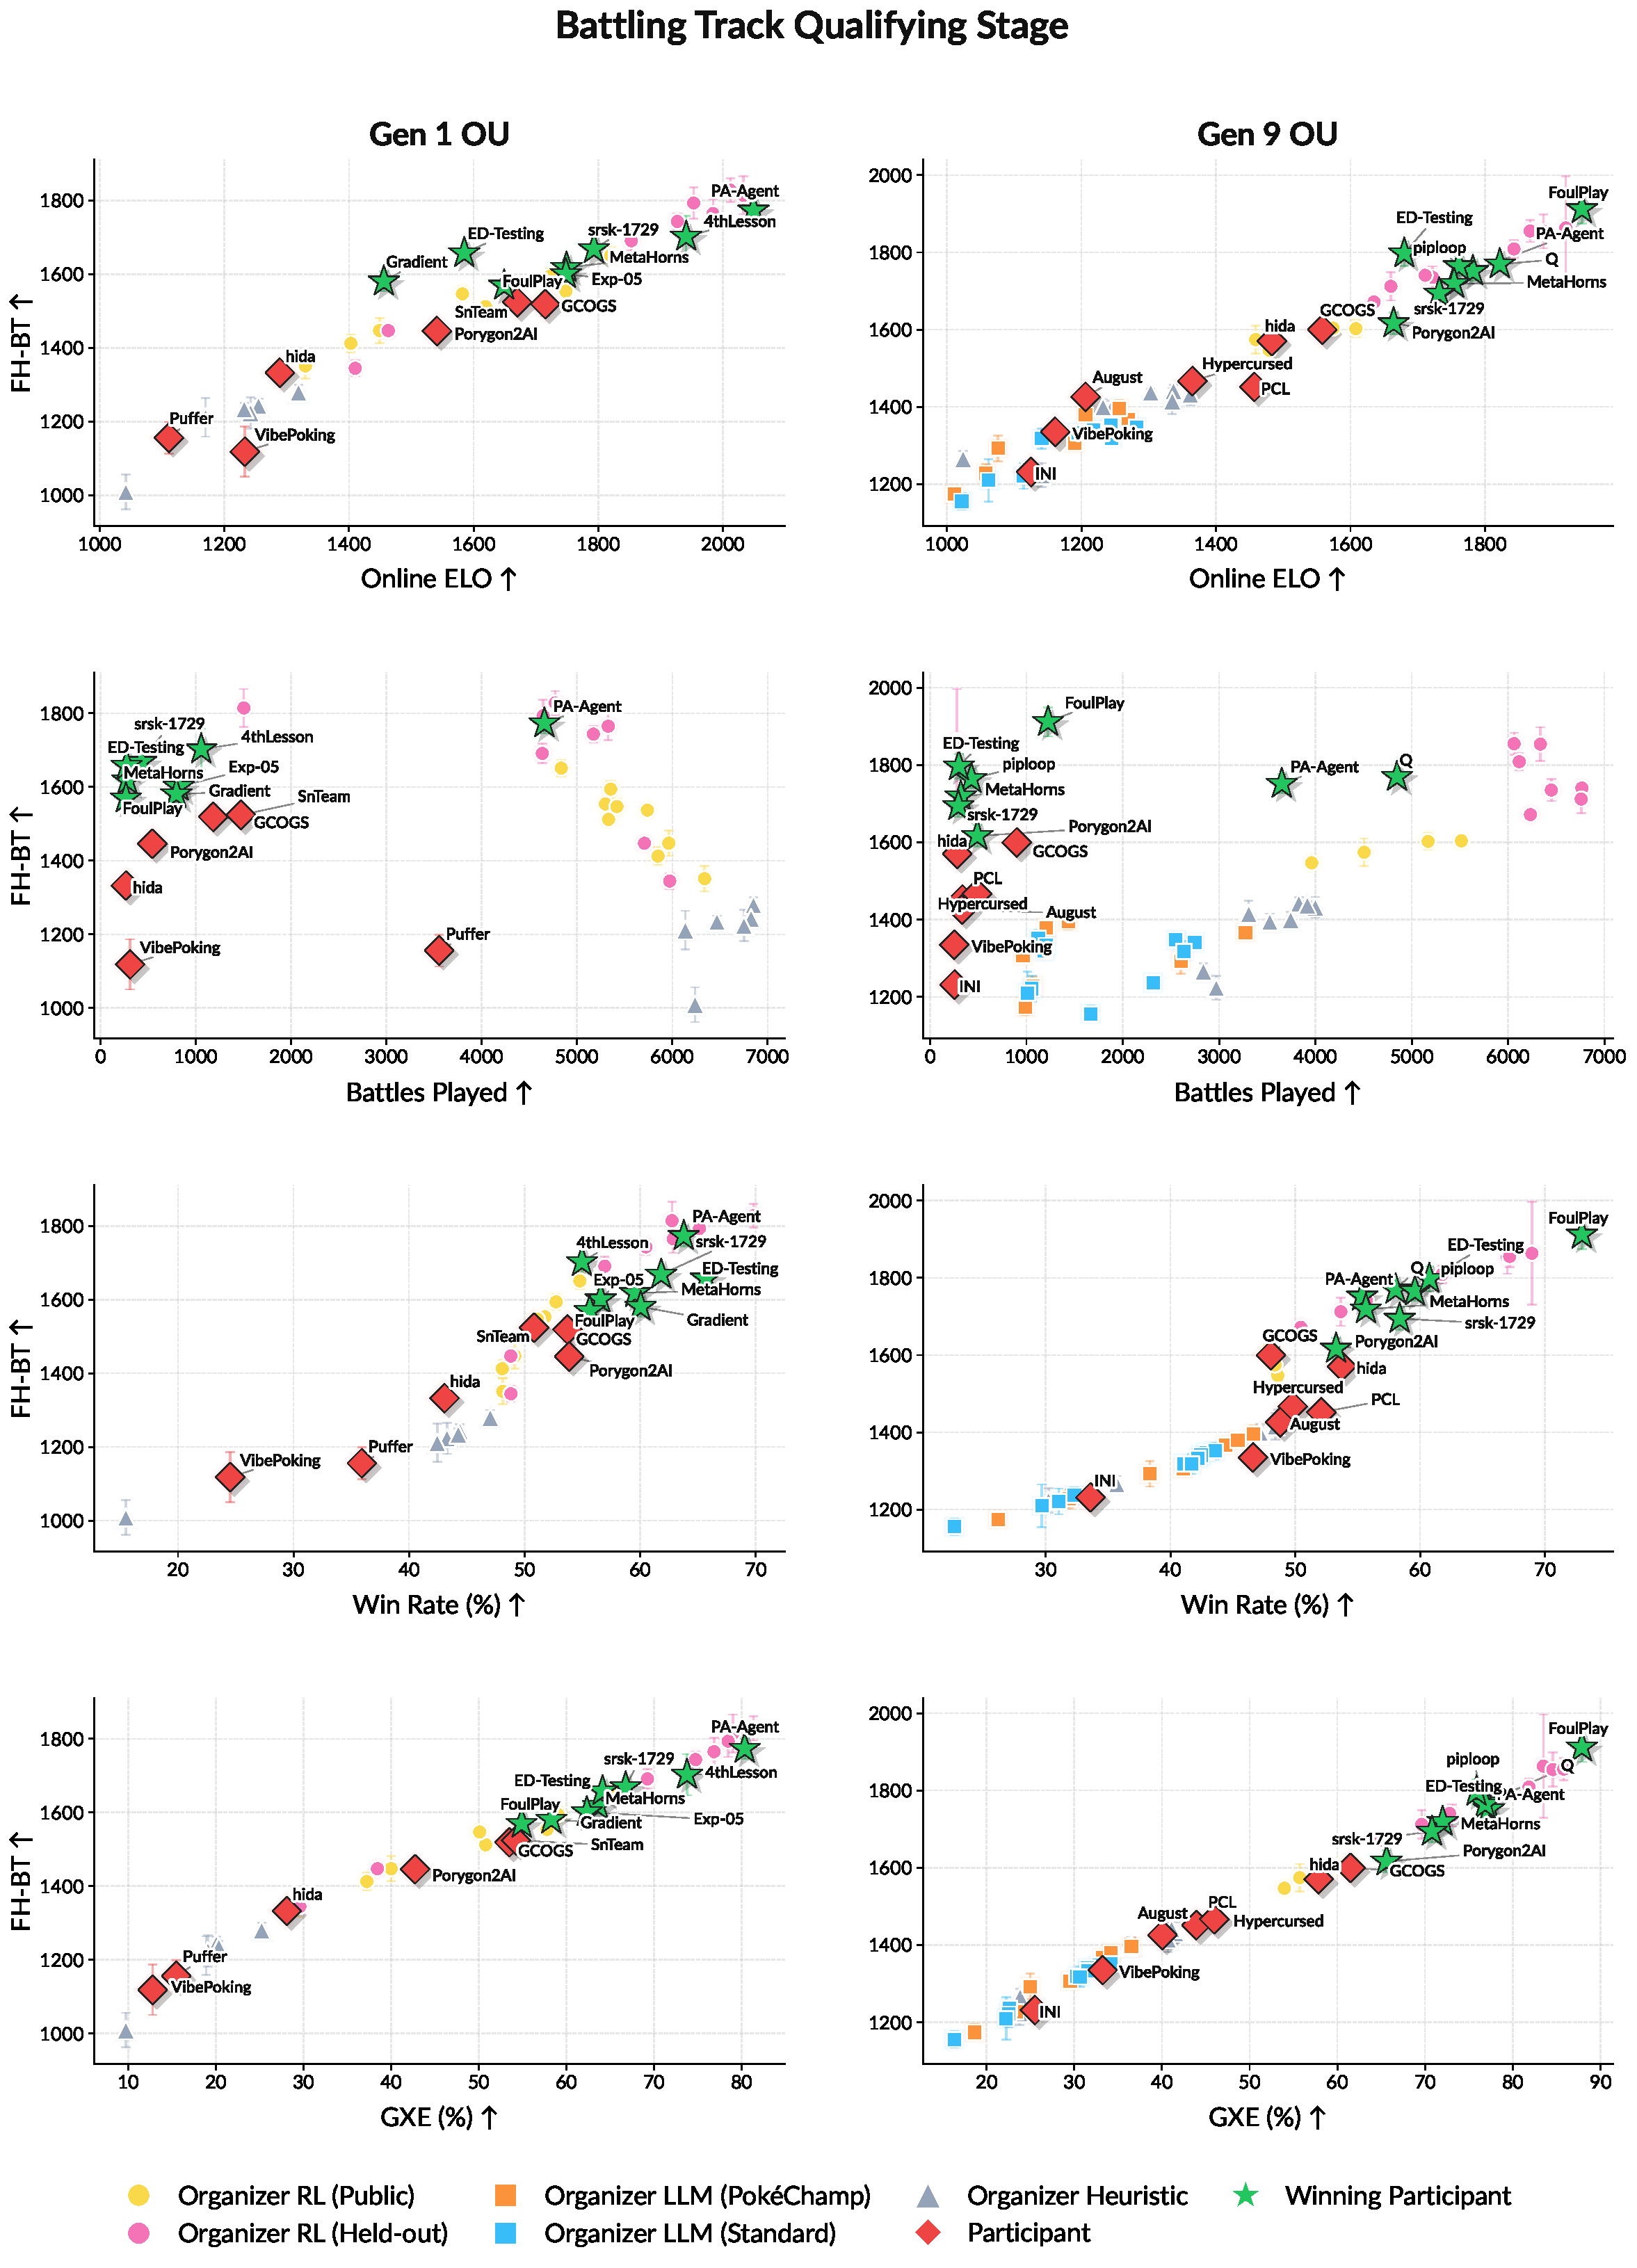
\includegraphics[width=\linewidth]{figures/track1_qualifying_scatter_appendix.pdf}
    \vspace{2mm}
    \caption{\textbf{Battling Track Qualifying Metrics.} Qualifying stage results according to alternative skill metrics (Showdown's Elo, GXE, Win Rate) and sample size (Battles Played). }
    \label{fig:track1_qualifying_scatter_appendix}
\end{figure}


\subsection{Judge's Choice Awards:}

The organizing committee awarded additional prizes based on participant technical writeups. These Judge's Choice awards were intended to reward novel directions and significant departures from the starter kit baselines regardless of final results. The winners were:
\begin{itemize}
    \item \textbf{\texttt{Porygon2AI}}: Recognized for innovative league training methodology inspired by AlphaStar's~\citep{vinyals2019grandmaster} approach to diverse opponent modeling
    \item \textbf{\texttt{August}}: Best pure LLM method without learned components, demonstrating effective chain-of-thought reasoning for move selection
\end{itemize}

